\section{Proposed Method}

This section presents the evaluated attention-enhanced lightweight framework. The objective is to test whether a single late CBAM block can improve a partially fine-tuned MobileNetV2 feature extractor without a large increase in model size. Mobile and edge deployment are treated as intended use cases that require separate hardware validation.

\subsection{Dataset Preparation}

The experiments use 54,306 PlantVillage images in 38 classes. Each class was partitioned independently with \texttt{train\_test\_split}: 70\% for training and 30\% temporary data, followed by an equal division of the temporary data into validation and test sets. Both operations used \texttt{random\_state=42}. The resulting directories contain 37,998 training images (69.97\%), 8,146 validation images (15.00\%), and 8,162 test images (15.03\%). Because the archived training notebooks additionally specified \texttt{validation\_split=0.2}, the fitted generators used 30,416 images from the training directory and 1,614 images from the validation directory; the test generator used all 8,162 test images. This legacy configuration is reported explicitly rather than being described as an 80/10/10 split.

Training images were rescaled to $[0,1]$ and augmented with rotations up to $25^{\circ}$, horizontal and vertical shifts of 0.2, zoom of 0.2, shear of 0.15, brightness factors from 0.8 to 1.2, horizontal flipping, and nearest-neighbor filling. Test images were only rescaled. MobileNetV2, MobileNetV2 + CBAM, and Xception used $224 \times 224$ inputs; InceptionV3 used its trained $299 \times 299$ input. A SHA-256 audit found no repeated filenames but identified 10 exact-image duplicate groups crossing directory splits; seven test images duplicated an image in training or validation. A sensitivity analysis therefore reports results both on all 8,162 test images and after excluding these seven test duplicates. The controlled acquisition conditions of PlantVillage---typically isolated leaves and uniform backgrounds---remain a limitation for field generalization.

\subsection{Overview of the Proposed Framework}

The proposed framework follows a transfer learning-based classification pipeline. Preprocessed images are passed through an ImageNet-pretrained MobileNetV2 backbone, the resulting convolutional feature maps are refined by sequential channel and spatial attention, and global average pooling plus a softmax layer produces the class probabilities.

The general workflow of the proposed framework can be summarized as follows:

\begin{equation}
    X \rightarrow F_{\text{MobileNetV2}}(X) \rightarrow F_{\text{CBAM}} \rightarrow F_{\text{GAP}} \rightarrow \hat{y},
\end{equation}

where $X$ denotes the input leaf image, $F_{\text{MobileNetV2}}(X)$ represents the feature maps extracted by the MobileNetV2 backbone, $F_{\text{CBAM}}$ denotes the attention-refined feature representation, $F_{\text{GAP}}$ represents global average pooling, and $\hat{y}$ is the predicted class probability distribution.

\begin{figure}[H]
\centering
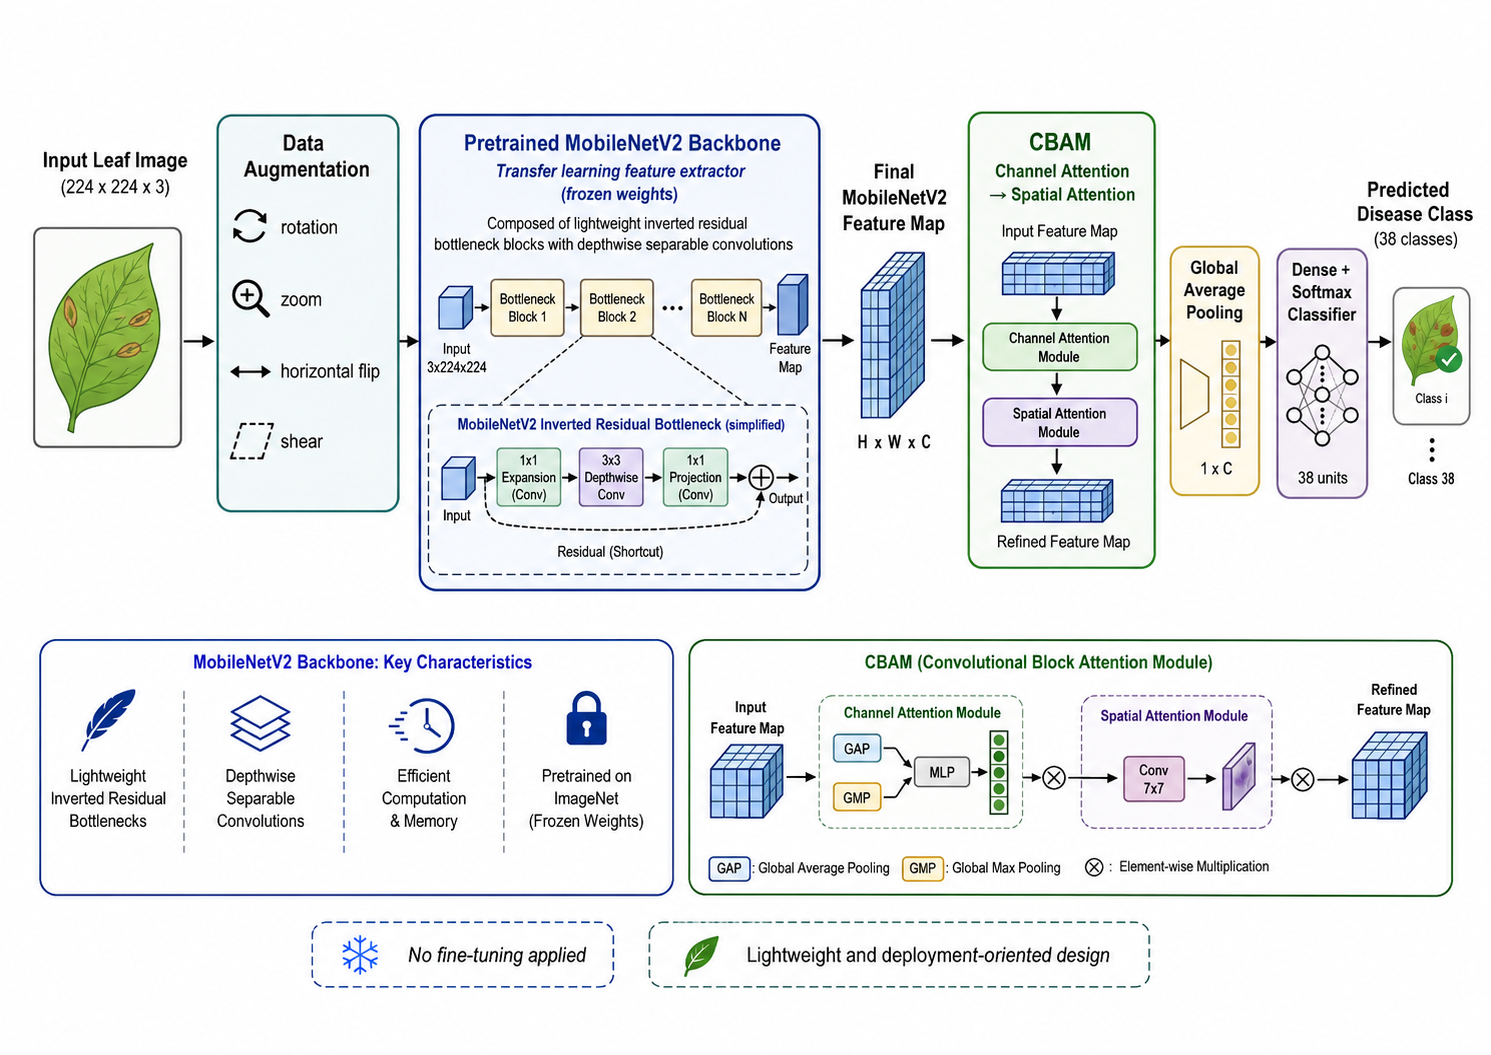
\includegraphics[width=0.95\textwidth]{figures/proposed_framework.png}
\caption{Overall architecture of the proposed attention-enhanced MobileNetV2 framework. CBAM is inserted after the final MobileNetV2 feature map and before global average pooling to refine channel and spatial feature representations.}
\label{fig:proposed_framework}
\end{figure}

\subsection{MobileNetV2 Backbone}

MobileNetV2 was selected because its inverted residual and linear-bottleneck design provides a well-established, readily convertible TensorFlow implementation with substantially fewer parameters than the heavier InceptionV3 and Xception comparators. This choice defines the present scope; it does not establish superiority over MobileNetV1, MobileNetV3, MobileNetV4, EfficientNet-B0, GhostNet, or ShuffleNetV2, which require a common-protocol comparison.

MobileNetV2 was selected as the baseline feature extraction architecture due to its lightweight design and suitability for mobile and embedded vision applications. Unlike conventional CNN architectures that rely heavily on standard convolutional operations, MobileNetV2 uses depthwise separable convolutions to reduce computational cost. A standard convolution applies filters across both spatial and channel dimensions simultaneously. In contrast, depthwise separable convolution decomposes this operation into a depthwise convolution followed by a pointwise convolution.

Given an input feature map, a standard convolution operation can be expressed as:

\begin{equation}
    Y = K * X,
\end{equation}

where $X$ is the input feature map, $K$ is the convolution kernel, $*$ denotes the convolution operation, and $Y$ is the output feature map.

In depthwise separable convolution, the depthwise convolution applies one spatial filter to each input channel independently:

\begin{equation}
    Y_{d}^{c} = K_{d}^{c} * X^{c},
\end{equation}

where $X^{c}$ is the $c$-th input channel, $K_{d}^{c}$ is the corresponding depthwise convolution kernel, and $Y_{d}^{c}$ is the resulting feature map for that channel. A pointwise convolution using $1 \times 1$ kernels is then applied to combine information across channels:

\begin{equation}
    Y = K_{p} * Y_{d},
\end{equation}

where $K_{p}$ represents the pointwise convolution kernel and $Y_{d}$ denotes the output of the depthwise convolution operation.

MobileNetV2 further improves efficiency through inverted residual blocks and linear bottlenecks~\cite{sandler2018mobilenetv2}. In an inverted residual block, the input feature representation is first expanded to a higher-dimensional space, processed using depthwise convolution, and then projected back to a lower-dimensional representation. The use of linear bottlenecks helps preserve useful information by avoiding non-linear activation in low-dimensional feature spaces. This design enables MobileNetV2 to maintain competitive classification performance while using fewer parameters and operations compared with heavier CNN architectures.

In this study, MobileNetV2 pretrained on ImageNet was used as the feature extraction backbone. The pretrained weights provide transferable low- and mid-level representations such as edges and textures. The backbone was initially frozen and its final 30 layers were then made trainable, providing limited task-specific adaptation while retaining most pretrained features.

\subsection{Convolutional Block Attention Module}

CBAM was selected because it combines channel selection (``what'' features) with spatial selection (``where'' features) in one sequential block. SE and ECA provide channel attention, whereas coordinate attention retains positional information through a different mechanism. The present experiment tests CBAM's two-dimensional refinement hypothesis; it does not claim superiority over those alternatives without a controlled attention-module ablation.

Although MobileNetV2 is computationally efficient, its lightweight structure may limit its ability to focus on subtle disease-specific regions in plant leaf images. Plant disease symptoms often appear as localized spots, color changes, or texture irregularities. Therefore, an attention mechanism can help improve feature discrimination by emphasizing informative regions and channels.

The Convolutional Block Attention Module (CBAM) is used in the proposed framework to refine the feature maps produced by MobileNetV2. CBAM applies attention sequentially along two dimensions: channel attention and spatial attention~\cite{woo2018cbam}. Channel attention identifies the most informative feature channels, while spatial attention highlights the most relevant spatial regions within the feature maps.

Given an intermediate feature map $F \in \mathbb{R}^{H \times W \times C}$, CBAM produces an attention-refined feature map $F''$ as follows:

\begin{equation}
    F' = M_c(F) \otimes F,
\end{equation}

\begin{equation}
    F'' = M_s(F') \otimes F',
\end{equation}

where $M_c(F)$ denotes the channel attention map, $M_s(F')$ denotes the spatial attention map, and $\otimes$ represents element-wise multiplication.

\subsubsection{Channel Attention}

The channel attention module determines which feature channels are most important for classification. It applies both global average pooling and global max pooling along the spatial dimensions of the input feature map. These operations generate two channel descriptors that summarize complementary information:

\begin{equation}
    F_{\text{avg}}^{c} = \text{AvgPool}(F),
\end{equation}

\begin{equation}
    F_{\text{max}}^{c} = \text{MaxPool}(F).
\end{equation}

The two descriptors are passed through a shared multilayer perceptron (MLP), and their outputs are combined and activated using a sigmoid function:

\begin{equation}
    M_c(F) = \sigma \left( \text{MLP}(F_{\text{avg}}^{c}) + \text{MLP}(F_{\text{max}}^{c}) \right),
\end{equation}

where $\sigma$ denotes the sigmoid activation function. The resulting channel attention map is multiplied with the input feature map to emphasize informative channels and suppress less relevant ones.

\subsubsection{Spatial Attention}

After channel attention, spatial attention is applied to identify important regions within the feature maps. Unlike channel attention, which focuses on the importance of feature channels, spatial attention focuses on where informative features are located. Average pooling and max pooling are applied along the channel dimension to produce two spatial descriptors:

\begin{equation}
    F_{\text{avg}}^{s} = \text{AvgPool}_{c}(F'),
\end{equation}

\begin{equation}
    F_{\text{max}}^{s} = \text{MaxPool}_{c}(F').
\end{equation}

These descriptors are concatenated and passed through a convolutional layer followed by a sigmoid activation:

\begin{equation}
    M_s(F') = \sigma \left( f^{7 \times 7} \left( [F_{\text{avg}}^{s}; F_{\text{max}}^{s}] \right) \right),
\end{equation}

where $f^{7 \times 7}$ denotes a convolution operation with a $7 \times 7$ kernel, and $[\cdot;\cdot]$ represents concatenation. The spatial attention map is then multiplied with the channel-refined feature map to obtain the final attention-enhanced representation.

\begin{figure}[H]
\centering
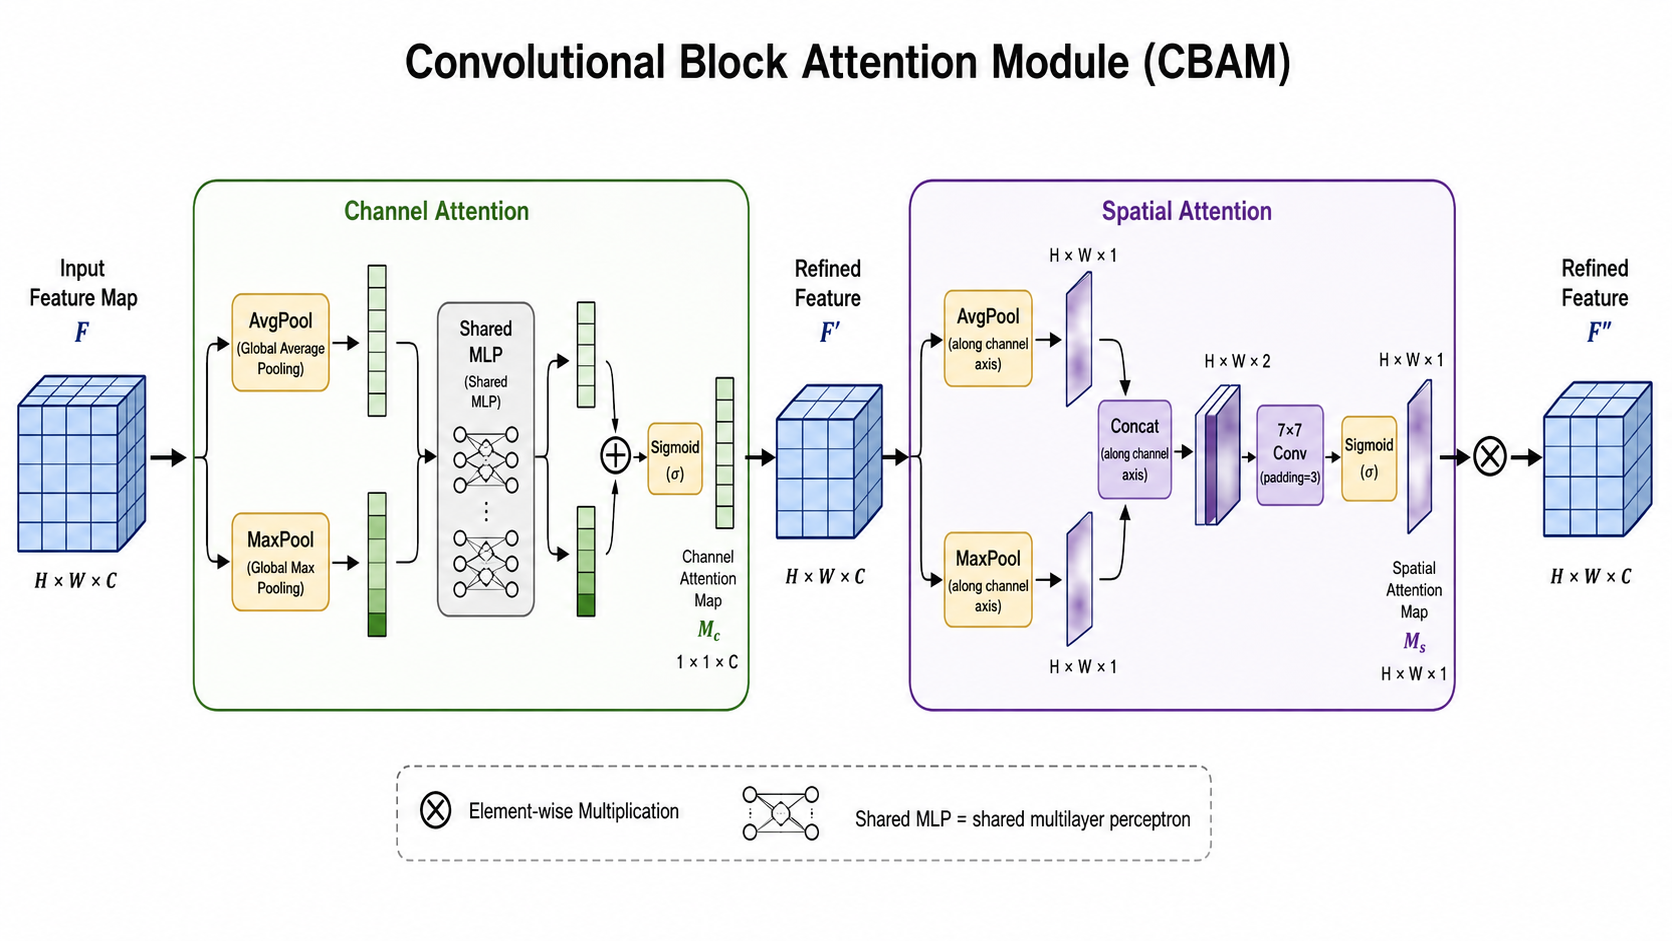
\includegraphics[width=0.90\textwidth]{figures/cbam_structure.png}
\caption{Structure of the Convolutional Block Attention Module. CBAM sequentially applies channel attention and spatial attention to refine the feature maps generated by the MobileNetV2 backbone.}
\label{fig:cbam_structure}
\end{figure}

\subsection{Integration of CBAM with MobileNetV2}

The late placement applies attention once to the most semantically developed convolutional map, avoiding repeated attention blocks throughout the backbone. It is a low-intervention design choice rather than a demonstrated optimum. The comparison with unmodified MobileNetV2 establishes its incremental cost, whereas early-, middle-, and post-pooling placements require a dedicated placement ablation.

In the proposed framework, CBAM is integrated after the final convolutional feature maps generated by the MobileNetV2 backbone and before the classification head. This integration strategy allows MobileNetV2 to first extract compact feature representations using its lightweight convolutional structure, after which CBAM refines these features by emphasizing disease-relevant channels and spatial regions.

Let $F_m$ denote the feature maps produced by the MobileNetV2 backbone:

\begin{equation}
    F_m = F_{\text{MobileNetV2}}(X).
\end{equation}

The CBAM module then refines these feature maps:

\begin{equation}
    F_a = \text{CBAM}(F_m),
\end{equation}

where $F_a$ represents the attention-enhanced feature map. The refined feature representation is passed through global average pooling:

\begin{equation}
    z = \text{GAP}(F_a).
\end{equation}

Finally, the output vector is passed to a dense classification layer with softmax activation:

\begin{equation}
    \hat{y}_i = \frac{e^{z_i}}{\sum_{j=1}^{K} e^{z_j}},
\end{equation}

where $\hat{y}_i$ is the predicted probability for class $i$, and $K$ is the total number of plant disease classes. In this study, $K=38$.

This design improves the representational capacity of MobileNetV2 while maintaining a lightweight architecture. By adding attention after feature extraction rather than replacing the backbone with a substantially heavier model, the proposed framework aims to balance classification accuracy and computational efficiency.

\subsection{Classification Head}

The classification head receives the attention-enhanced feature representation and maps it to the final disease classes. After CBAM refinement, global average pooling is applied to reduce the spatial dimensions of the feature maps while retaining channel-wise information. A dense layer with softmax activation is then used to produce the final class probability distribution.

The classification objective is optimized using categorical cross-entropy loss, defined as:

\begin{equation}
    \mathcal{L} = - \sum_{i=1}^{K} y_i \log(\hat{y}_i),
\end{equation}

where $y_i$ is the ground-truth label for class $i$, $\hat{y}_i$ is the predicted probability for class $i$, and $K$ is the number of classes. Since the dataset contains multiple plant disease categories, categorical cross-entropy is appropriate for the multi-class classification setting.

\subsection{Transfer Learning Strategy}

All models in this study were trained using transfer learning. The convolutional backbones were initialized with ImageNet pretrained weights, while the task-specific classification layers were trained on the PlantVillage dataset. Transfer learning was used to reduce training time and improve convergence by leveraging visual representations learned from large-scale image data.

For each backbone, all layers were first frozen and the final 30 layers were then unfrozen. The attention block and classification head were also trainable. This common partial-fine-tuning rule allowed deeper features to adapt to disease texture and morphology while limiting optimization cost. It also corrects the earlier description of the backbones as completely frozen. The present study does not compare different unfreezing depths; such an ablation remains necessary to establish whether 30 layers provide the best accuracy--cost trade-off.

\subsection{Proposed Model Summary}

The proposed MobileNetV2 + CBAM framework is designed to provide a balanced trade-off between classification performance and computational efficiency. MobileNetV2 contributes a compact and efficient feature extraction backbone, while CBAM enhances the extracted representations through channel and spatial attention. The model is therefore intended to improve the baseline lightweight architecture without introducing the high computational cost typically associated with deeper CNNs.

The key stages of the proposed method are summarized as follows:

\begin{enumerate}
    \item Input leaf images are resized to $224 \times 224$ pixels.
    \item Data augmentation is applied during training using rotation, zoom, horizontal flipping, and shear transformation.
    \item MobileNetV2 pretrained on ImageNet extracts lightweight convolutional feature maps.
    \item CBAM refines the extracted feature maps using sequential channel and spatial attention.
    \item Global average pooling converts the refined feature maps into a compact feature vector.
    \item A softmax classification layer predicts one of the 38 plant disease classes.
\end{enumerate}

\begin{table}[H]
\caption{Summary of the proposed MobileNetV2 + CBAM architecture.}
\label{tab:proposed_model_summary}
\centering
\begin{tabularx}{\textwidth}{p{3.0cm} p{4.0cm} X}
\toprule
\textbf{Stage} & \textbf{Component} & \textbf{Description} \\
\midrule
Input & Leaf image & Resized to $224 \times 224 \times 3$. \\
\addlinespace
Feature extraction & MobileNetV2 backbone & ImageNet-pretrained lightweight CNN with the final 30 layers unfrozen. \\
\addlinespace
Attention refinement & CBAM & Sequential channel and spatial attention applied to the final MobileNetV2 feature maps. \\
\addlinespace
Feature aggregation & Global Average Pooling & Converts the refined feature maps into a compact feature vector. \\
\addlinespace
Classification & Dense + Softmax & Predicts one of 38 healthy or diseased plant leaf classes. \\
\bottomrule
\end{tabularx}
\end{table}
